\begin{quote}
Perfection is achieved\\only on the point of collapse.\\- C. N. Parkinson
\end{quote}

\section{Analogietabelle}

%Wegen Build Fehlern, ein '\:' vor jedem '\downarrow' entfernt

\begin{center}
\begin{tabular}{l|l|l}
\text{Translation} &  & \text{Rotation}\\\hline
\(\vec{s}\) &  & \(\vec{\varphi}\)\\
\(\downarrow\frac{ds}{dt}\) &  & \(\downarrow \frac{d\varphi}{dt}\)\\
\(\vec{v}\) & \(\vec{v}=\vec{\omega} \times \vec{r}\) & \(\vec{\omega}\)\\
\(\downarrow\frac{dv}{dt}\) &  & \(\downarrow \frac{d\omega}{dt}\)\\
\(\vec{a}\) & \(a = \underbrace{\alpha \times r}_{a_{Tan}} - \underbrace{\omega^2 r}_{a_R}\) & \(\vec{\alpha}\)\\\hline
m &  & J\\
\(\downarrow \frac{dm}{dt}\) &  & \(\downarrow \frac{dJ}{dt}\)\\
\(\vec{F}\) &  & \(\vec{M}\)\\
\(\downarrow \frac{dF}{dt}\) &  & \(\downarrow \frac{dM}{dt}\)\\
\(\vec{p}\) &  & \(\vec{L}\)\\
\(\frac{m}{2}v^2\) & \(E_{kin}\) & \(\frac{J}{2}\omega^2\)
\end{tabular}
\end{center}

\newpage
\begin{multicols}{2}{}
\subsection{Translation}

\begin{align*}
	a(t)&=a_0=\frac{\diff v}{\diff t}=\dot{v}=\ddot{s} \\
	v(t)&=a_0\cdot t+v_0=\frac{\diff s}{\diff t}=\dot{s} \\
	s(t)&=\frac{1}{2}a_0\cdot t^2+v_0\cdot t+s_0
\end{align*}

\subsection{Rotation}

\begin{align*}
\alpha(t)&=\alpha_0=\frac{\diff \omega}{\diff t}=\dot{\omega}=\ddot{\varphi} \\
\omega(t)&=\alpha_0\cdot t+\omega_0=\frac{\diff \varphi}{\diff t}=\dot{\varphi} \\
\varphi(t)&=\frac{1}{2}\alpha_0\cdot t^2+\omega_0\cdot t+\varphi_0
\end{align*}
\end{multicols}

\begin{multicols}{2}{}
\subsubsection*{Bahngroessen}
\begin{align*}
a_t(t)&=a_0=\frac{\diff v}{\diff t}=\dot{v}=\ddot{s} \\
v(t)&=a_0\cdot t+v_0=\frac{\diff s}{\diff t}=\dot{s} \\
s(t)&=\frac{1}{2}a_0\cdot t^2+v_0\cdot t+s_0
\end{align*}


\subsubsection*{Winkelgroessen}
\begin{align*}
\vec{a_t}	&=\vec{\alpha} \times \vec{r} =\alpha\cdot r \qquad \alpha \perp r \\
\vec{\alpha}	&=\vec{r} \times \vec{a_t}\\
\vec{v}		&=\vec{\omega}\times\vec{r} =\omega\cdot r  \qquad \omega \perp r\\
\vec{\omega}	&=\vec{r} \times \vec{v}\\
s		&=\varphi\cdot r  
\end{align*}
\end{multicols}        


\begin{multicols}{2}{}
\subsubsection*{Kreisfrequenz}
\begin{align*}
\omega&=\frac{2\cdot\pi}{T}\\
&=2\cdot\pi\cdot n \\
&=2\cdot\pi\cdot f
\end{align*}


\subsubsection*{Radialbeschleunigung}
\begin{align*}
a_r&=\frac{v^2}{r}\\
&=v\cdot\omega\\
&=\omega^2\cdot r
\end{align*}
\end{multicols}


\subsubsection*{Umdrehungen}
\begin{align*}
N&=\frac{\omega_0\cdot t}{2\cdot \pi}+\frac{1}{2}\cdot\frac{\alpha}{2\cdot \pi}\cdot t^2\\
&=n_0\cdot t+\frac{\alpha}{4\cdot\pi}\cdot t^2
\end{align*}


\newpage
\section{Dynamik}

\subsection{Geradlinig (Translation)}
\begin{align*}
\vec{F}&=m\cdot \vec{a}\\
\vec{F}_{\text{Tr}}&=-m\cdot \vec{a}
\end{align*}
\begin{multicols}{2}{}
\subsubsection*{Impuls}
\begin{align*}
\vec{p}&=m\cdot \vec{v}\\ \\
\end{align*}

\subsubsection*{Kraftstoss}
\begin{align*}
\vec{F}&=\frac{\diff \vec{p}}{\diff t}=m\cdot\frac{\diff \vec{v}}{\diff t}+\vec{v}\cdot\frac{\diff m}{\diff t}\\
\Delta\vec{p}&=\vec{p}_2-\vec{p}_1=\int_{\vec{p}_2}^{\vec{p}_1}\diff p=\int_0^{t}\vec{F}\diff t
\end{align*}
\end{multicols}

\begin{multicols}{2}{}
\subsubsection*{Arbeit}
\begin{align*}
W&=-\int_{\vec{s}_1}^{\vec{s}_2}\vec{F_{\text{Tr}}}\circ\diff \vec{s}\\
&=\int_{\vec{v}_0}^{\vec{v}_1}m\vec{v}\circ\diff \vec{v}=\frac{1}{2}m\left(v_1^2-v_0^2\right) 
\end{align*}

\subsubsection*{Hubarbeit}
\begin{align*}
W_{\text{hub}}&=mgh
\end{align*}
\end{multicols}

\begin{multicols}{2}{}
\subsubsection*{Kinetische Energie}
\begin{align*}
E_{\text{kin}}=\frac{1}{2}mv^2
\end{align*}

\subsubsection*{Leistung}
\begin{align*}
P=\vec{F}\circ\vec{v}=\frac{\diff W}{\diff t}=\dot{W}
\end{align*}
\end{multicols}


\subsection{Drehbewegung(Rotation)}

\begin{multicols}{2}{}
\subsubsection*{Massentraegheitsmoment}
\begin{align*}
J=\int r^2 \diff m
\end{align*}

\subsubsection*{Drehmoment}
\begin{align*}
\vec{M}&=\vec{r}\times\vec{F}=J\vec{\alpha}=\dot{\vec{L}}
\end{align*}
\end{multicols}

\begin{multicols}{2}{}
\subsubsection*{Drehimpuls}
\begin{align*}
\vec{L}&=\vec{r}\times\vec{p} \\
&=J\cdot \vec{\omega}
\end{align*}

\subsubsection*{Kinetische Energie}
\begin{align*}
E_{kin}=\frac{1}{2}J\omega^2 \\
\end{align*}
\end{multicols}

\begin{multicols}{2}{}
\subsubsection*{Arbeit}
\begin{align*}
W &=\int_{\varphi_0}^{\varphi_1}\vec{M}\circ\vec{e_\omega}\diff \varphi \\
&=\int_{\vec{\omega}_0}^{\vec{\omega}_1}J\vec{\omega}\diff\vec{\omega}\\
&=\frac{1}{2}J\left(\omega_1^2-\omega_0^2\right)
\end{align*}

\subsubsection*{Leistung}
\begin{align*}
P=\vec{M}\circ\vec{\omega}
\end{align*}

\subsubsection*{Zentripedalkraft}
\begin{align*}
F_{zp}&=-m\cdot\omega^2\cdot r\\
&=-m\cdot v^2\cdot \frac{\vec{e_r}}{r}
\end{align*}
\end{multicols}


\subsection{Geneigte Ebene}

\subsubsection*{Kräfte}
\begin{align*}
\vec{F}_N&=\vec{F}_G\cos\alpha\\
\vec{F}_H&=\vec{F}_G\sin\alpha
\end{align*}


\subsection{Reibung}

\begin{multicols}{2}{}
\subsubsection*{Reibungskraft}
\begin{align*}
F_R=\mu\cdot F_N
\end{align*}
\vfill
\subsubsection*{Rollreibung}
\begin{align*}
M&=f\cdot F_N\\
F_R&=\frac{f}{r}\cdot F_N
\end{align*}
\vfill
\end{multicols}

\newpage
\subsection{Feder}

\begin{multicols}{2}{}
\subsubsection*{HOOKsches Gesetz}
\begin{align*}
F&=-kx\\
M&=D\varphi
\end{align*}

\subsubsection*{Federspannarbeit}
\begin{align*}
W	&=\int_{x_\text{min}}^{x_\text{max}}F\diff x=\int_{x_\text{min}}^{x_\text{max}}kx\diff x\\
	&=\frac{1}{2}\cdot k\cdot \left(x_{\text{max}}^2-x_{\text{min}}^2\right)
\end{align*}
\end{multicols}

\subsection{Elastischer Stoss}

\begin{align*}
\text{Energie vor den Stoß} &= \text{Energie nach den Stoß}\nonumber\\
\sum E_{\text{kin}}&=\sum E_{\text{kin}}'
\end{align*}


\subsubsection*{Impulserhaltung}
\begin{align*}
\text{Impuls vor den Stoß} &= \text{Impuls nach den Stoß}\nonumber\\
\sum m\vec{v}&= \sum m\vec{v}'
\end{align*}


\subsubsection*{Zentraler, Gerader, Elastischer Stoss}
\begin{align*}
\frac{1}{2}m_1v_1^2+\frac{1}{2}m_2v_2^2&=\frac{1}{2}m_1v_1'^2+\frac{1}{2}m_2v_2'^2\\
m_1v_1+m_2v_2&=m_1v_1'+m_2v_2'
\end{align*}

\begin{align*}
v_2'&=\frac{2m_1}{m_1+m_2}v_1+\frac{m_2-m_1}{m_1+m_2}v_2\\
v_1'&=\frac{2m_2}{m_1+m_2}v_2+\frac{m_1-m_2}{m_1+m_2}v_1
\end{align*}


\subsection{Unelastischer Stoss}

\subsubsection*{Energieerhaltung}
\begin{align*}
\text{Energie vor den Stoß} &= \text{Energie nach den Stoß}+\text{Arbeit}\nonumber\\
\sum E_{\text{kin}}&=\sum E_{\text{kin}}'+\Delta W
\end{align*}


\subsubsection*{Impulserhaltung}
\begin{align*}
\text{Impuls vor den Stoß} &= \text{Impuls nach den Stoß}\nonumber\\
\sum m\vec{v}&= \sum m\vec{v}'
\end{align*}


\subsubsection*{Total unelastischer Stoss}
\begin{align*}
\frac{1}{2}m_1v_1^2+\frac{1}{2}m_2v_2^2&=\frac{1}{2}\left(m_1+m_2\right)v'^2+\Delta W\\
m_1v_1+m_2v_2&=\left(m_1+m_2\right)v'
\end{align*}

\begin{align*}
v'&=\frac{m_1v_1+m_2v_2}{m_1+m_2}
\end{align*}

\begin{align*}
\Delta W	&=\frac{m_1\cdot m_2}{2\left(m_1+m_2\right)}\left(v_1-v_2\right)^2
\end{align*}



\subsubsection*{Drehimpulserhaltungssatz}
\begin{align*}
\text{Drehinpuls zur Zeit 1} &= \text{Drehimpuls zur Zeit 2}\\
\sum \vec{L}&=\sum \vec{L}'
\end{align*}


\subsubsection*{Kopplung zweier Rotationskörper}
\begin{align*}
\vec{\omega}'&=\frac{J_0\vec{\omega_0}+J_1\vec{\omega_1}}{J_1+J_2}\\
W&=\frac{J_0\cdot J_1}{2\left(J_0+J_1\right)}\left(\omega_0-\omega_1\right)^2
\end{align*}


\subsection{Rotierendes Bezugssystem}

\begin{multicols}{2}{}
\subsubsection*{Zentrifugalkraft}
\begin{align*}
\vec{F}_Z&=F_r\cdot \vec{e}_r=-m\vec{\omega}\times\left(\vec{\omega}\times\vec{r}\right)\\
&=-m\vec{\omega}\times\vec{v}\\
F_Z&=-m\frac{v^2}{r}=-m\omega^2 r
\end{align*}


\subsubsection*{Corioliskraft}
\begin{align*}
\vec{F}_C&=-2m\vec{\omega}\times\vec{v}
\end{align*}
\vspace{10mm}
\end{multicols}

\section{Schwerpunkt}

\begin{multicols}{2}{}
\subsection*{mehrere Punktmassen}
\begin{align*}
\vec{r}_{\text{Sp}}=\frac{\sum\vec{r}_i m_i}{\sum\ m_i}
\end{align*}


\subsection*{Allgemein}
\begin{align*}
\vec{r}_{\text{Sp}}=\frac{\int \vec{r}\diff m}{\int \diff m}
\end{align*}
\end{multicols}

\begin{multicols}{2}{}
\subsubsection*{Schwerpunkt in \\Zylinderkoordinaten}
\begin{align*}
r_{\text{Sp}}&=\frac{\int_z\int_\varphi\int_r r^2\rho \diff r \diff \varphi \diff z }{\int_z\int_\varphi\int_r r\rho \diff r \diff \varphi \diff z }\\
\varphi_{\text{Sp}}&=\frac{\int_z\int_\varphi\int_r \varphi r\rho \diff r \diff \varphi \diff z }{\int_z\int_\varphi\int_r r\rho \diff r \diff \varphi \diff z }\\
z_{\text{Sp}}&=\frac{\int_z\int_\varphi\int_r z r\rho \diff r \diff \varphi \diff z }{\int_z\int_\varphi\int_r r\rho \diff r \diff \varphi \diff z }\\
x&=r\cos{\varphi}\hspace{3mm}y=r\sin{\varphi}\hspace{3mm}z=z
\end{align*}

\subsubsection*{Schwerpunkt in \\karthesischen Koordinaten}
\begin{align*}
x_{\text{Sp}}&=\frac{\int_z\int_y\int_x x\rho \diff x \diff y \diff z }{\int_z\int_y\int_x \rho \diff x \diff y \diff z }\\
y_{\text{Sp}}&=\frac{\int_z\int_y\int_x y\rho \diff x \diff y \diff z }{\int_z\int_y\int_x \rho \diff x \diff y \diff z }\\
z_{\text{Sp}}&=\frac{\int_z\int_y\int_x z\rho \diff x \diff y \diff z }{\int_z\int_y\int_x \rho \diff x \diff y \diff z }
\end{align*}
\hfill
\end{multicols}


\newpage
\section{Trägheitsmoment}


\begin{align*}
J&=\sum m_i r_i^2\\
J&=\int_m r^2 \diff m \\
J&=\int_z\int_\varphi\int_r r^3\rho \diff r \diff \varphi \diff z 
\end{align*}

\begin{multicols}{2}{}
\subsubsection*{STEINER'scher Satz}
\begin{align*}
J_x&=mr^2+J_s
\end{align*}

%Tabelle einf�gen
\subsubsection*{Traegheitsmoment Kugel}
\begin{align*}
J_\text{Sp}&=\frac{2}{5}mr^2
\end{align*}


\subsubsection*{Traegheitsmoment Zylinder}
\begin{align*}
J_\text{Sp}&=\frac{1}{2}mr^2
\end{align*}


\subsubsection*{Traegheitmoment Kreisring \\(Torus)}
\begin{align*}
J_\text{Sp}&=mr^2
\end{align*}


\subsubsection*{Traegheitsmoment Stab}
\begin{align*}
J_\text{Sp}=\frac{1}{12}ml^2
\end{align*}
\end{multicols}


\newpage
\section{Elastizitaetslehre}

\begin{multicols}{2}{}
\subsubsection*{Spannung}
\begin{align*}
\vec{\sigma}&=\frac{\diff\vec{F}_n}{\diff A}\\
\sigma&=E \varepsilon=E\frac{\Delta l}{l}\\
\vec{\tau}&= \frac{\diff\vec{F}_t}{\diff A}
\end{align*}
\hfill

\begin{center}
 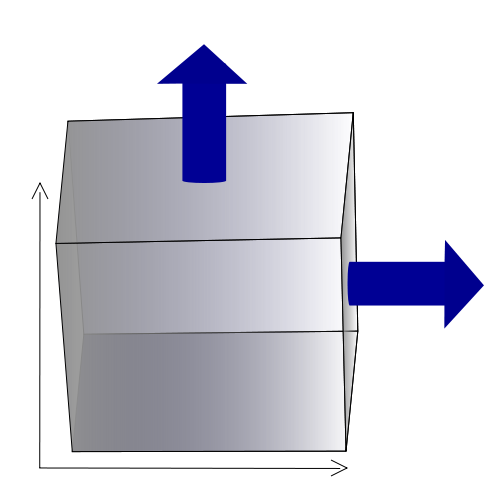
\includegraphics[width=40mm,height=40mm,keepaspectratio=true]{./Physik/Bilder/Spannung.png}
\end{center}
\end{multicols}


\subsubsection*{Schubmodul}

\begin{multicols}{2}{}
\begin{align*}
G&=\frac{\tau}{\varphi}
\end{align*}
\hfill

\begin{center}
 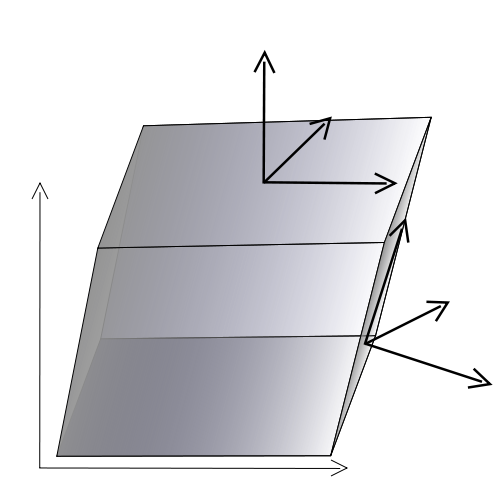
\includegraphics[width=40mm,height=40mm,keepaspectratio=true]{./Physik/Bilder/Tangentialspannung.png}
\end{center}
\end{multicols}


\subsubsection*{Drillung}

\begin{multicols}{2}{}
\begin{align*}
\psi&=\frac{\diff \varphi}{\diff l}=\frac{W_t}{G\cdot J_p}\tau=\frac{M_t}{G\cdot J_p}
\end{align*}
\hfill

\begin{center}
 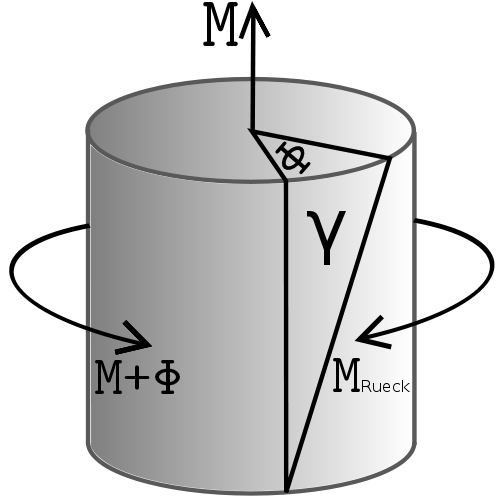
\includegraphics[width=40mm,height=40mm,keepaspectratio=true]{./Physik/Bilder/Scherbeanspruchung.png}
\end{center}
\end{multicols}


\begin{multicols}{2}{}
\subsubsection*{Flaechenmoment}
\begin{align*}
J_p&=\int r^2\diff A=\int_\varphi\int_r r^3\diff r \diff \varphi 
\end{align*}


\subsubsection*{Verformungsarbeit}
\begin{align*}
W&=V\int \sigma(\varepsilon) \diff \varepsilon 
\end{align*}
\end{multicols}


\section{Schwingungen}


\subsubsection*{Harmonische Schwingungen}
\begin{align*}
u(t)=A\cos(\omega t+\varphi_0)
\end{align*}


\subsection{Ungedämpfte Schwingungen}

\begin{align*}
\ddot{x}&=-\frac{k}{m}x\\
x(t)&=\hat{x}\cos(\omega_0 t+\varphi_0)\\
\dot{x}(t)&=-\hat{x}\omega\sin(\omega_0 t+\varphi_0)\\
\ddot{x}(t)&=-\hat{x}\omega^2\cos(\omega_0 t+\varphi_0)\\
\omega&=\sqrt{\frac{k}{m}}\\
f&=\frac{1}{2\pi}\sqrt{\frac{k}{m}}\\
T&=2\pi\sqrt{\frac{m}{k}}
\end{align*}

\newpage
\begin{multicols}{2}{}
\subsubsection*{Mathemetisches Pendel}
\begin{align*}
\ddot{\varphi}&=-\frac{g}{l}\varphi\\
\varphi(t)&=\hat{\varphi}\cos(\omega_0 t+\varphi_0)\\
\dot{\varphi}(t)&=-\hat{\varphi}\omega\sin(\omega_0 t+\varphi_0)\\
\ddot{\varphi}(t)&=-\hat{\varphi}\omega^2\cos(\omega_0 t+\varphi_0)\\
\omega&=\sqrt{\frac{g}{l}}\\
f&=\frac{1}{2\pi}\sqrt{\frac{g}{l}}\\
T&=2\pi\sqrt{\frac{l}{g}}
\end{align*}

\subsubsection*{Physikalisches Pendel}
\begin{align*}
\ddot{\varphi}&=-\frac{lmg}{J_A}\varphi\\
\varphi(t)&=\hat{\varphi}\cos(\omega_0 t+\varphi_0)\\
\dot{\varphi}(t)&=-\hat{\varphi}\omega\sin(\omega_0 t+\varphi_0)\\
\ddot{\varphi}(t)&=-\hat{\varphi}\omega^2\cos(\omega_0 t+\varphi_0)\\
\omega&=\sqrt{\frac{mgl}{J_A}}\\
f&=\frac{1}{2\pi}\sqrt{\frac{mgl}{J_A}}\\
T&=2\pi\sqrt{\frac{J_A}{mgl}}
\end{align*}
\end{multicols}

\begin{multicols}{2}{}
\subsubsection*{Torsionsschwingung}
\begin{align*}
\ddot{\varphi}&=-\frac{D}{J_A}\varphi\\
\varphi(t)&=\hat{\varphi}\cos(\omega_0 t+\varphi_0)\\
\dot{\varphi}(t)&=-\hat{\varphi}\omega\sin(\omega_0 t+\varphi_0)\\
\ddot{\varphi}(t)&=-\hat{\varphi}\omega^2\cos(\omega_0 t+\varphi_0)\\
\omega&=\sqrt{\frac{D}{J_A}}\\
f&=\frac{1}{2\pi}\sqrt{\frac{D}{J_A}}\\
T&=2\pi\sqrt{\frac{J_A}{D}}
\end{align*}



\subsubsection*{Flüssigkeitspendel}
\begin{align*}
\ddot{y}&=-\frac{2A\rho g}{m}y\\
\varphi(t)&=\hat{y}\cos(\omega_0 t+\varphi_0)\\
\dot{\varphi}(t)&=-\hat{y}\omega\sin(\omega_0 t+\varphi_0)\\
\ddot{\varphi}(t)&=-\hat{y}\omega^2\cos(\omega_0 t+\varphi_0)\\
\omega&=\sqrt{\frac{2A\rho g}{m}}=\sqrt{\frac{2g}{l}}\\
f&=\frac{1}{2\pi}\sqrt{\frac{2g}{l}}\\
T&=2\pi\sqrt{\frac{l}{2g}}
\end{align*}
\end{multicols}

\begin{multicols}{2}
\subsubsection*{Elektrischer Schwingkreis}
\begin{align*}
0&=L\ddot{Q}+\frac{Q}{C}\\
q(t)&=\hat{Q}\cos(\omega_0 t+\varphi_0)\\
\dot{q}(t)&=-\hat{Q}\omega\sin(\omega_0 t+\varphi_0)\\
\ddot{q}(t)&=-\hat{Q}\omega^2\cos(\omega_0 t+\varphi_0)\\
\omega&=\sqrt{\frac{1}{LC}}\\
f&=\frac{1}{2\pi}\sqrt{\frac{1}{LC}}\\
T&=2\pi\sqrt{\frac{1}{LC}}
\end{align*}
\vfill
\end{multicols}


\subsection{Gedaempfte Schwingungen}

\begin{multicols}{2}{}
\subsubsection*{Schwingungsgleichung}
\begin{align*}
m\ddot{x}=-kx+F_R
\end{align*}
\hfill

\subsubsection*{COULOMB Reibung}
\begin{align*}
F_R&=-\operatorname{sgn}({\dot{x}})\mu F_N\\
0&=m\ddot{x}+kx+\operatorname{sgn}({\dot{x}})\mu F_N\\
\end{align*}
\end{multicols}


\subsubsection*{Gleitreibung}
\begin{align*}
x(t)&=-(\hat{x}_0-\hat{x}_1)\cos(\omega t)-\hat{x}_1\qquad 0\leq t\leq \frac{T}{2}\\
x(t)&=-(\hat{x}_0-3\hat{x}_1)\cos(\omega t)+\hat{x}_1\qquad \frac{T}{2}\leq t\leq T\\
\hat{x}_1&=\frac{\mu F_N}{k}
\end{align*}


\subsubsection*{Viskosereibung}
\begin{multicols}{2}{}
\begin{align*}
0&=m\ddot{x}+b\dot{x}+kx\\
x(t)&=\hat{x}e^{-\delta t}e^{\pm j\sqrt{\omega_0^2-\delta^2}t}\\
x(t)&=\hat{x}e^{-\delta t}e^{\pm j\omega_0\sqrt{1-D^2}t}\\
\delta&=\frac{b}{2m}\\
D&=\frac{\delta}{\omega_0}\\
D&=\frac{b}{2}\frac{1}{\sqrt{mk}}\\
\omega_0&=\sqrt{\frac{k}{m}}\\
\Lambda&=\ln\left(\frac{x(t)}{x(t+T)}\right)\\
\Lambda&=\delta T\\
\omega_D&=\sqrt{\frac{k}{m}-\left(\frac{b}{2m}\right)^2}\\
d&=2D\\
Q&=\frac{1}{d}
\end{align*}

{
\begin{align*}
x(t)&=\hat{x}e^{-\delta t}\cos(\sqrt{\omega_0^2-\delta^2}t+\varphi)\\
\end{align*}

\begin{align*}
&\text{Aperiodischer Grenzfall $\delta=\omega_0$}\\
&x(t)=\hat{x}e^{-\delta t}(1-\delta t)
\end{align*}

\begin{align*}
&\text{Kriechfall $\delta>\omega_0$}\\
&x(t)=\hat{x}e^{-\delta t}e^{\pm j\sqrt{\omega_0^2-\delta^2}t}
\end{align*}
}
\hfill

\end{multicols}